
\chapter{Customization}

\section{Command history}

Append the following commands into your shell init file: (mine is ~/.zshrc)


\lstset{language=Sh}
\begin{lstlisting}
  
# history config
export HISTSIZE=100000 # history commands nums
export HISTCONTROL=ignoredups # ignore duplicated commands

\end{lstlisting}



\section{Emacs dired icloud directory}

\subsection{Customize MacOS}

\verb|System Preferences| $\rightarrow$
\verb|Security & Privacy| $\rightarrow$
\verb|Privacy| $\rightarrow$
\verb|Full Disk Access| $\rightarrow$
add \verb|Emacs.app| into it.

\begin{figure}[!ht]
  \centering
  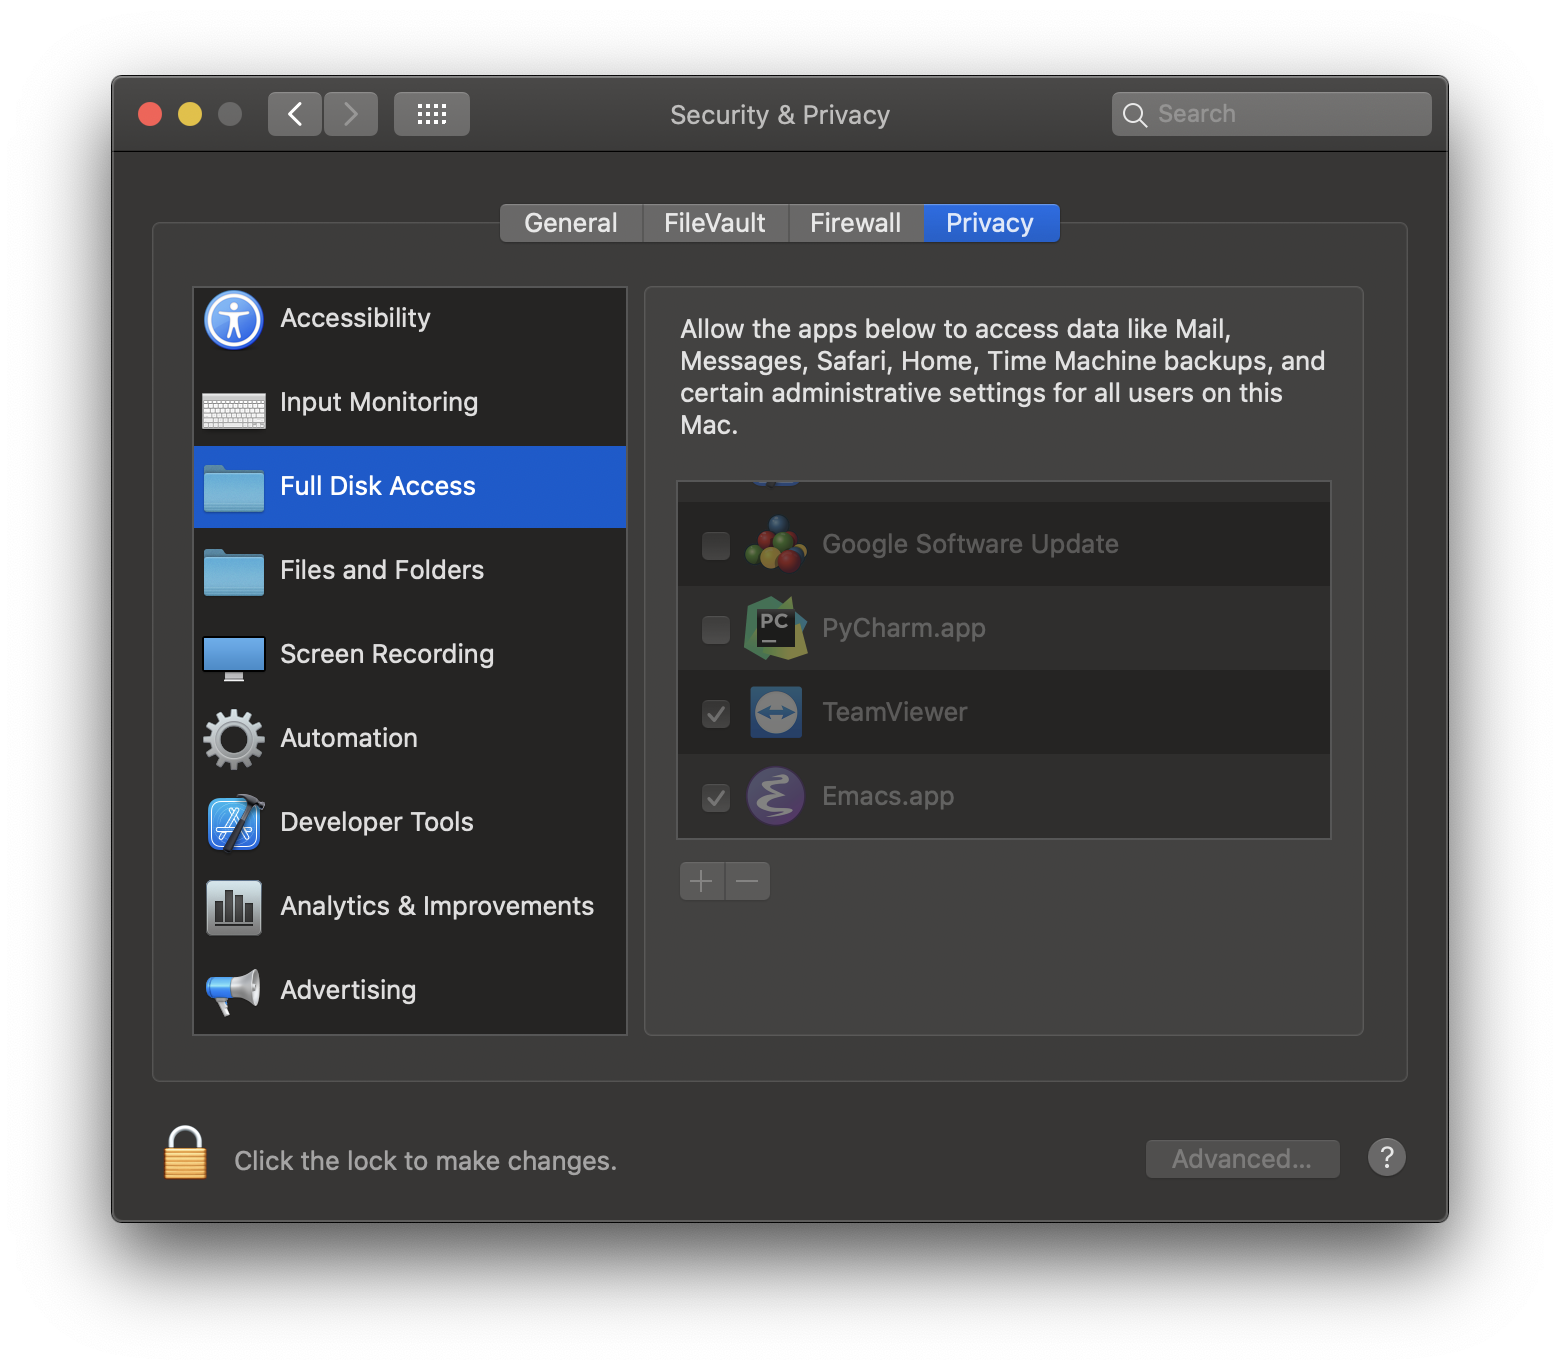
\includegraphics[width=\textwidth]{pics/emacs-full-disk-access}
  \caption{Emacs full disk access}
  \label{fig:emacs-full-disk-access}
\end{figure}

As shown in Figure \ref{fig:emacs-full-disk-access}.


\subsection{First visit icloud directory}

The first time to visit the icloud directory, you should use
\verb|M-x ns-open-file-using-panel| to open the icloud directory.
After that, you can access the icloud directory.
